%==============================================================================
% Sjabloon poster bachproef
%==============================================================================
% Gebaseerd op document class `a0poster' door Gerlinde Kettl en Matthias Weiser
% Aangepast voor gebruik aan HOGENT door Jens Buysse en Bert Van Vreckem

\documentclass[a0,portrait]{hogent-poster}

% Info over de opleiding
\course{Bachelorproef}
\studyprogramme{toegepaste informatica}
\academicyear{2023-2024}
\institution{Hogeschool Gent, Valentin Vaerwyckweg 1, 9000 Gent}

% Info over de bachelorproef
\title{Onderzoek naar pentesting binnen specifieke webomgevingen}
\author{Levi Van Achter}
\email{levi.vanachter@student.hogent.be}
\supervisor{Benjamin Vertonghen }
\cosupervisor{Stijn D'Hollander (Sinergio)}

% Indien ingevuld, wordt deze informatie toegevoegd aan het einde van de
% abstract. Zet in commentaar als je dit niet wilt.
\specialisation{Mobile & Enterprise developmen}
\keywords{Penetratietesten, Webapplicaties, Beveiliging, Ethical Hacking, Cybersecurity}
%\projectrepo{https://github.com/user/repo}

\begin{document}

\maketitle

\begin{abstract}
  Dit onderzoek richt zich specifiek op penetratietesten binnen een webomgeving, waarbij de focus ligt op het
  identificeren en beveiligen van kwetsbaarheden in webapplicaties. Het omvat een grondige verkenning van
  methodologieën en technieken die worden toegepast bij het testen van de beveiliging van webapplicaties. Het
  onderzoek analyseert populaire webgerichte aanvalsvectoren zoals SQL-injecties, cross-site scripting (XSS),
  brute force.... Daarnaast wordt een vergelijkende studie uitgevoerd om de effectiviteit van
  de testen op meten bij 3 verschillende we applicaties
\end{abstract}

\begin{multicols}{2} % This is how many columns your poster will be broken into, a portrait poster is generally split into 2 columns

\section{Introductie}

Cybersecurity is een cruciaal, maar vaak onderbelicht aspect binnen softwareontwikkeling. Deze bachelorproef onderzoekt 
de effectiviteit van verschillende penetratietesttools op basis van gestelde criteria. De uitgekomen tool zal de vergelijking 
maken tussen drie specifieke webomgevingen: een WordPress-omgeving zonder beveiligingsplugins, een WordPress-omgeving met 
beveiligingsplugins, en een Laravel-applicatie.

Door gestructureerde penetratietests met tools zoals Burp Suite, OWASP ZAP en Metasploit, worden kwetsbaarheden in elke 
omgeving geanalyseerd en beoordeeld. De resultaten tonen aan dat de WordPress-
omgeving zonder beveiligingsplugins het meest kwetsbaar is, terwijl de Laravel- en WordPress-applicatie moeilijker te 
vergelijken zijn met elkaar door een gelijkaardige basissecurity, maar verschillende bijkomende optionele secuty. 
Een WordPress website wordt vaak gebruikt voor een snelle en gemakkelijke opzet, terwijl een Laravel-applicatie meer 
geschikt is voor op maat gemaakte applicaties.

Daarnaast blijken Burp Suite en OWASP ZAP zeer gebruiksvriendelijk te zijn, terwijl Metasploit uitblinkt in diepgaande 
testmogelijkheden. Dit onderzoek benadrukt de noodzaak van effectieve beveiligingsstrategieën en biedt praktische 
aanbevelingen voor de selectie en implementatie van penetratietesttools in softwareprojecten.

\section{Experimenten}

In dit hoofdstuk worden de experimenten beschreven die zijn uitgevoerd met de verkozen pentesttool OWASP 
ZAP. Deze tool is uitgevoerd op een WordPress-omgeving zonder beveiligingsplugins, 
een WordPress-omgeving met beveiligingsplugins, en een Laravel-applicatie.

Uit voorop gestelde criteria werd OWASP ZAP gekozen als meest effectieve tool voor het identificeren van kwetsbaarheden 
deze criteria waren: efficiëntie, functionaliteiten, kostprijzen, resourceverbruik, ondersteuning van de community en 
beoordeling van derden. OWASP ZAP scoorde hoog op deze criteria en werd daarom gekozen voor de experimenten.

De reeks experimenten betrof het gebruik van OWASP ZAP in de WordPress-omgeving met beveiligingsplugins. 
Hierbij werden zes specifieke aanvallen uitgevoerd die gekozen zijn op basis van de owasp top 10 lijst. Zo zijn 
de volgende vulnerabilities getest een brute force attack, een SQL-injectie, sensitive data exposure, security 
misconfiguration, cross-site scripting en insufficient logging and monitoring. Deze tests waren 
gericht op het identificeren van kwetsbaarheden ondanks de aanwezigheid van beveiligingsplugins.

\begin{center}
  \captionsetup{type=figure}
  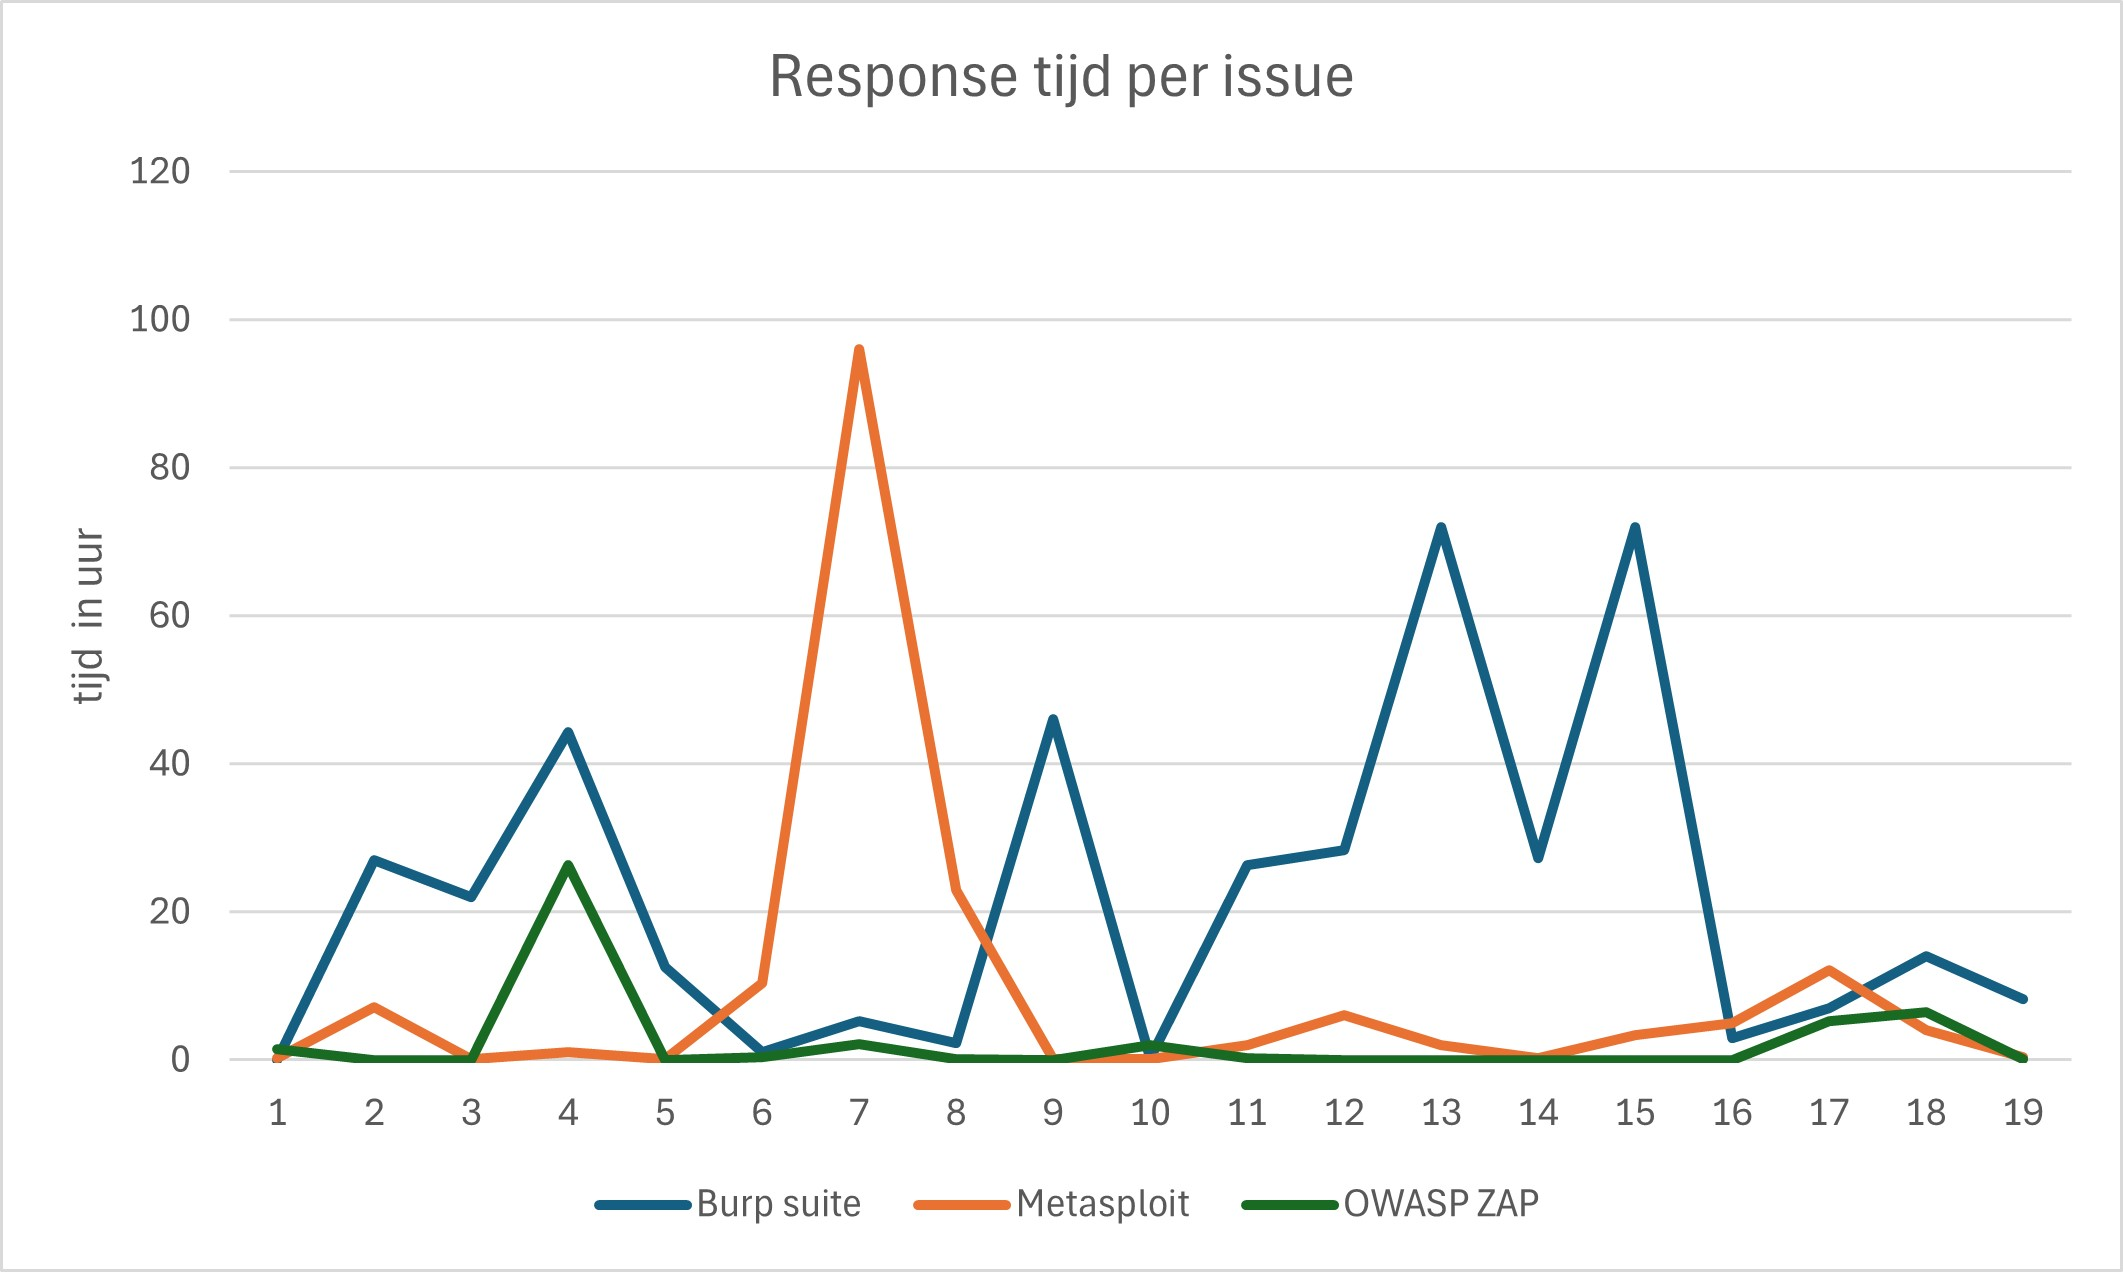
\includegraphics[width=1.0\linewidth]{grafiek_respons_resultaten.jpg}
  \captionof{figure}{Respons tijd resultaten van de experimenten voor pentest-tool keuze}
\end{center}


\section{Conclusies}

De prestaties van OWASP ZAP varieerden veel bij het identificeren van kwetsbaarheden in de 
drie specifieke webomgevingen. Bij brute force-aanvallen op een WordPress-omgeving zonder de Wordfence-plugin 
slaagden geen van de tool erin om ongelimiteerdte proberen in te loggen. Bij de SQL-injectie werd elk script als gereflecteerd 
beschouwd, wat aantoont dat de SQL-injectie-aanvallen een mogelijke bedreiging kan vormen. Bij security misconfiguration 
werd een kwetsbaarheid op vlak van weergegeven meldingen bij het ingeven van een juiste gebruikersnaam en een foutief wahtwoord.

In een WordPress-omgeving met de Wordfence-plugin werd door de tool minder kwetsbaarheden blootgelegd. 
De Wordfence-plugin zorgde voor een aanzienlijke verbetering in het detecteren en blokkeren van aanvallen 
zoals brute force-aanvallen en security misconfiguration. De ingebouwde beveiligingsmaatregelen van de plugin, zoals geavanceerde 
het blokkeren van een gebruiker na een aantal foutieve inlogpogingen en het weergeven van een correcte melding bij een foutief wachtwoord 
en correcte gebruikersnaam, boden een solide bescherming. Bij de SQL-injectie werden slechts enkele script als gereflecteerd beschouwt.

De Laravel-applicatie toonde een vergelijkbare weerstand tegen aanvallen, wat de geavanceerde, ingebouwde beveiligingsmaatregelen van 
het framework benadrukt. Buiten bij de SQL-injectie werden er geen scripts als gereflecteerd beschouwt.

De overige kwetsbaarheden werden niet gedetecteerd door de tools of testen op de omgevingen, maar door externe testen op de 
server en database. De conclusie hierbij is voor elke omgeving hetzelfde, doordat dit een kwetsbaarheid is die niet door de tool 
kan worden gedetecteerd. Zo wer de cross-site scripting en sensitive data exposure niet gedetecteerd door de tool, aangezien dit regels zijn 
die ingesteld worden op server en database niveau. Ook de insufficient logging and monitoring werd niet gedetecteerd door de tool, 
maar door externe testen op de server en database.

Beveiligingsplugins verbeterden de detectiecapaciteiten van de tools aanzienlijk. Ze beperkten het aantal inlogpogingen, 
vergrendelden accounts na overschrijding van de limiet en stuurden real-time alerts bij verdachte activiteiten. OWASP ZAP 
en de betaalde versie van Burp Suite detecteerden bekende kwetsbaarheden met hoge efficiëntie.
\begin{center}
  \captionsetup{type=figure}
  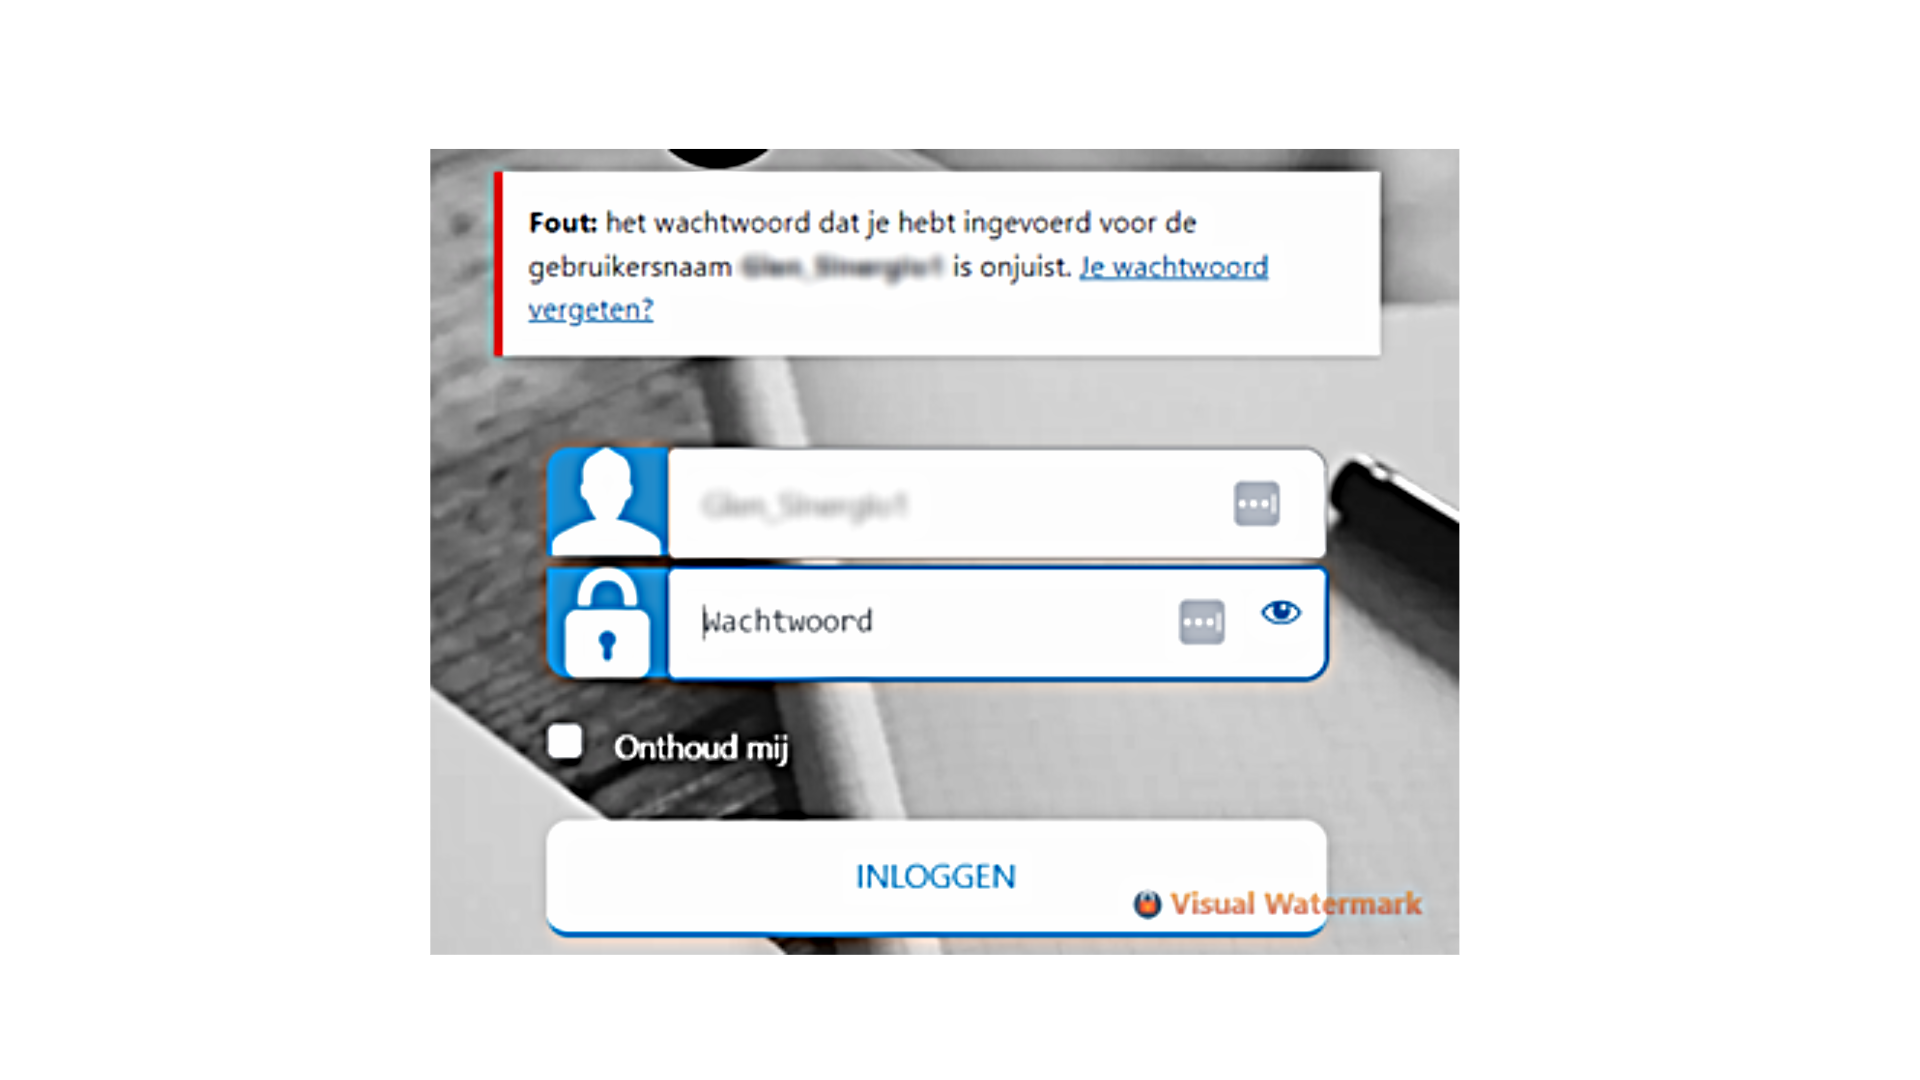
\includegraphics[width=1\linewidth]{Naamloos.png}
  \captionof{figure}{melding bij het ingeven van een foutief wachtwoord en correcte gebruikersnaam}
\end{center}
\section{Toekomstig onderzoek}

Voor toekomstig onderzoek zijn er verschillende interessante mogelijkheden om de bevindingen van deze studie verder uit te 
breiden. Een belangrijk aspect dat nog nader onderzocht kan worden, is het gebruik van de Burp Suite Professional Edition. 
Deze versie biedt uitgebreidere functionaliteiten en diepgaandere analyseopties dan de Community Edition, waardoor een extra 
vergelijking kan worden gemaakt met andere penetratietesttools zoals Metasploit en OWASP ZAP.

Daarnaast kunnen toekomstige studies zich richten op het testen van nieuwe beveiligingsplugins en updates binnen de 
WordPress- en Laravel-omgevingen. Het is essentieel om te evalueren hoe deze verbeteringen de effectiviteit van bestaande 
beveiligingsmaatregelen beïnvloeden en of ze nieuwe kwetsbaarheden introduceren.
\end{multicols}
\end{document}